\chapter{Relativistische kinematica}\label{ch:b3:relativistic-kinematics}

Kosmische straling die de hoge atmosfeer treft maakt op vijftien
kilometer hoogte muonen --- onstabiele deeltjes die gemiddeld twee
microseconden leven. Twee microseconden bij bijna de lichtsnelheid is
zeshonderd meter; toch tikken muondetectoren op zeeniveau gestaag door en
tellen zij deeltjes die twintig keer hun toegemeten bereik hebben
afgelegd. De oplossing van deze paradox is geen detail uit de
deeltjesfysica, maar een herziening van de begrippen onder de hele
natuurkunde: de tijd verstrijkt voor het bewegende muon anders dan voor
ons, en afstanden krimpen langs zijn beweging. Dit hoofdstuk bouwt die
herziening --- de speciale relativiteitstheorie (Einstein, 1905) --- op
uit haar twee postulaten: de wetten van de natuurkunde zijn in elk
\omterm{thm:b3:relativistic-kinematics:postulates}{inertiaalstelsel} dezelfde, en licht in vacuüm heeft in alle
\omterm{thm:b3:relativistic-kinematics:postulates}{inertiaalstelsels} dezelfde snelheid. De rest volgt uit eerlijke
kinematica: de verstrengeling van ruimte met tijd in de
\omterm{thm:b3:relativistic-kinematics:lorentz}{lorentztransformatie}, de rek van de tijd, de krimp van lengten, de nieuwe
regel voor het samenstellen van snelheden, en de meetkunde --- de
ruimtetijd en haar invariante interval --- waarin dat alles even
vanzelfsprekend wordt als een rotatie.

\section{Twee postulaten tegen de absolute tijd}

\begin{remark}[Waar het conflict vandaan komt]\label{rem:b3:relativistic-kinematics:conflict}
De mechanica heeft altijd al een relativiteitsbeginsel gehad: in een
rustig varend schip verraadt geen enkele proef met ballen en slingers de
beweging (Galilei), en de wetten van Newton gelden in elk
\emph{\omterm{thm:b3:relativistic-kinematics:postulates}{inertiaalstelsel}}, de stelsels die ten opzichte van elkaar met
constante snelheid bewegen. Maar het elektromagnetisme van het volume van
jaar 2 leidt uit natuurconstanten een welbepaalde lichtsnelheid af, $c = 1/\sqrt{\varepsilon_0\mu_0} =
\qty{3.00e8}{m/s}$, zonder te vermelden wie
haar meet --- en de proeven bevestigen het: de snelheid van sterrenlicht
dat op de bewegende aarde aankomt, door de seizoenen heen gemeten,
verandert nooit (Michelson en Morley, 1887, en elke opvolger sindsdien).
De kinematica van Galilei, waarin snelheden optellen, kan een snelheid
die voor iedereen dezelfde is niet verteren. Er moet iets wijken, en dat
is onze aanname dat tijd en \omterm{def:b3:relativistic-kinematics:event}{gelijktijdigheid} absoluut zijn.
\end{remark}

\begin{theorem}[De postulaten van de speciale relativiteitstheorie]\label{thm:b3:relativistic-kinematics:postulates}
\index{relativiteit!postulaten}\index{inertiaalstelsel}
\emph{(i) Relativiteit:} de wetten van de natuurkunde nemen in elk
\omterm{thm:b3:relativistic-kinematics:postulates}{inertiaalstelsel} dezelfde vorm aan; geen enkele proef onderscheidt rust
van eenparige beweging. \emph{(ii) Licht:} licht in vacuüm plant zich in
elk \omterm{thm:b3:relativistic-kinematics:postulates}{inertiaalstelsel} met dezelfde snelheid $c$ voort, wat de beweging van
de bron of de waarnemer ook is.
\end{theorem}
\admitted

\begin{definition}[Gebeurtenissen en gelijktijdigheid]\label{def:b3:relativistic-kinematics:event}
\index{gebeurtenis}\index{gelijktijdigheid}
Een \emph{gebeurtenis} is een puntvormig voorval: een bepaalde plaats
\emph{én} een bepaald ogenblik --- een vonk, een tik van een detector,
een verval. Elk \omterm{thm:b3:relativistic-kinematics:postulates}{inertiaalstelsel} kent een gebeurtenis de coördinaten
$(t, x, y, z)$ toe met meetlatten die in het stelsel rusten en
gelijkgezette klokken die erover verdeeld staan. Twee gebeurtenissen
heten \emph{gelijktijdig in een stelsel} wanneer de klokken van dat
stelsel er dezelfde $t$ aan toekennen --- en het eerste slachtoffer van
de postulaten is dat dit begrip van het stelsel afhangt.
\end{definition}

\begin{example}[De trein en de twee bliksemschichten]\label{ex:b3:relativistic-kinematics:train}
De bliksem slaat in aan beide uiteinden van een snelle trein en laat
sporen na op trein en spoor. Voor de waarneemster op de grond, midden
tussen de sporen, komen de twee flitsen samen aan: voor haar waren de
inslagen gelijktijdig. De passagier die op het midden van de trein zit,
beweegt echter naar de ene flits toe en van de andere weg; omdat ook in
zijn stelsel het licht met $c$ loopt, bereikt de voorste flits hem
eerder --- en omdat hij even ver van de twee sporen \emph{op de trein}
zit, moet hij besluiten dat de voorste inslag \emph{eerder} plaatsvond.
Geen van beiden heeft ongelijk: de \omterm{def:b3:relativistic-kinematics:event}{gelijktijdigheid} van gescheiden
gebeurtenissen is geen feit over de wereld maar over het stelsel. Elke
relativistische ``paradox'' lost hier op.
\end{example}

\begin{omfigure}
\begin{tikzpicture}[font=\small, >=Stealth]
  % ground view
  \begin{scope}
    \draw[thick] (-0.3,0) -- (10.3,0);
    \fill[omDef!18, draw=omDef, thick, rounded corners=2pt] (1.4,0.15) rectangle (8.6,1.05);
    \foreach \x in {2.2,3.4,4.6,5.8,7.0} \draw[omDef] (\x,0.35) rectangle (\x+0.7,0.85);
    \draw[->, very thick] (8.9,0.6) -- (9.9,0.6) node[right] {$v$};
    \node[omExo] at (1.4,1.75) {\Large$\downarrow$};
    \node[omExo] at (8.6,1.75) {\Large$\downarrow$};
    \node[omExo, font=\footnotesize] at (1.4,2.15) {inslag A};
    \node[omExo, font=\footnotesize] at (8.6,2.15) {inslag B};
    \fill (5,-0.02) circle (2pt);
    \node[font=\footnotesize] at (5,-0.4) {waarneemster op de grond, in het midden};
    \fill[omThm] (5,1.22) circle (2pt);
    \node[omThm, font=\footnotesize] at (5.1,1.55) {passagier, midden op de trein};
  \end{scope}
\end{tikzpicture}

{\small Twee inslagen die zowel de trein als het spoor merken. De
waarneemster op de grond, midden tussen de sporen, ontvangt de flitsen
samen: voor haar gelijktijdig. De passagier loopt flits B tegemoet; die
bereikt hem eerder, en --- even ver van de sporen in zijn eigen stelsel
--- besluit hij dat B het eerst insloeg. \omterm{def:b3:relativistic-kinematics:event}{Gelijktijdigheid} is relatief.}
\end{omfigure}

\section{De lorentztransformatie}

\begin{theorem}[Lorentztransformatie]\label{thm:b3:relativistic-kinematics:lorentz}
\index{lorentztransformatie}\index{gammafactor@$\gamma$-factor}
Laat het stelsel $\mathcal R'$ met snelheid $v$ langs de $x$-as van het
stelsel $\mathcal R$ bewegen, met samenvallende oorsprongen op $t = t' = 0$. Een \omterm{def:b3:relativistic-kinematics:event}{gebeurtenis} $(t, x)$ van $\mathcal R$ heeft in $\mathcal R'$ de
coördinaten
\[
x' = \gamma\,(x - vt) , \qquad
t' = \gamma\Big(t - \frac{v\,x}{c^2}\Big) , \qquad
\gamma = \frac{1}{\sqrt{1 - v^2/c^2}} ,
\]
met $y' = y$, $z' = z$; de omgekeerde transformatie is dezelfde met
$v \to -v$. Voor $v \ll c$ gaat $\gamma \to 1$ en vindt men Galilei's
$x' = x - vt$, $t' = t$ terug. De factor $\gamma \ge 1$ --- nauwelijks
$1$ bij alledaagse snelheden, $1.15$ bij $c/2$, $7.1$ bij $0.99c$ ---
meet elk relativistisch effect van dit hoofdstuk.
\end{theorem}

\begin{proof}[Gedeeltelijk bewijs]
De homogeniteit van ruimte en tijd dwingt de transformatie lineair te
zijn; de symmetrie tussen de stelsels en het relativiteitspostulaat
herleiden haar tot $x' = \gamma(x - vt)$, $x = \gamma(x' + vt')$ met één
onbekende functie $\gamma(v)$. Volg een lichtflits die in de
gemeenschappelijke oorsprong wordt uitgezonden: postulaat (ii) eist $x = ct$ \emph{en} $x' = ct'$. Invullen geeft $ct' = \gamma t(c - v)$ en $ct = \gamma t'(c + v)$; vermenigvuldiging van de twee vergelijkingen geeft
$c^2 = \gamma^2(c^2 - v^2)$, wat de aangegeven $\gamma$ is. Eliminatie
van $x'$ tussen de twee lineaire betrekkingen levert de tijdformule. (De
stap van ``het licht klopt'' naar ``de hele transformatie ligt vast'' ---
geen resterende rek van de dwarsrichtingen of herschaling --- gebruikt de
symmetrieargumenten van \cref{exo:b3:relativistic-kinematics:11}.)
\end{proof}

\begin{proposition}[Tijdrek]\label{prop:b3:relativistic-kinematics:dilation}
\index{tijdrek}\index{eigentijd}
Een klok die in $\mathcal R'$ rust --- die tikt bij vaste $x'$ --- loopt
gezien vanuit $\mathcal R$ achter: tussen twee van haar tikken, gescheiden
door de \emph{\omterm{prop:b3:relativistic-kinematics:dilation}{eigentijd}} $\Delta\tau$ (de tijd van het stelsel waarin de
klok rust), meet het stelsel $\mathcal R$
\[
\Delta t = \gamma\,\Delta\tau \ge \Delta\tau .
\]
Bewegende klokken lopen traag --- alle, biologische, atomaire of
subatomaire, want het is de tijd zelf die rekt, geen mechaniek.
\end{proposition}

\begin{proof}
Twee tikken bij dezelfde $x'$: de omgekeerde transformatie geeft $\Delta t
= \gamma(\Delta t' + v\,\Delta x'/c^2) = \gamma\,\Delta\tau$ omdat
$\Delta x' = 0$. Het beeld van de lichtklok
(\cref{exo:b3:relativistic-kinematics:2}) levert dezelfde $\gamma$ uit
Pythagoras alleen.
\end{proof}

\begin{proposition}[Lengtekrimp]\label{prop:b3:relativistic-kinematics:contraction}
\index{lengtekrimp}\index{eigenlengte}
Een staaf met \emph{\omterm{prop:b3:relativistic-kinematics:contraction}{eigenlengte}} $L_0$ (haar lengte in haar ruststelsel)
die in de lengterichting met $v$ beweegt, meet in het laboratorium
\[
L = \frac{L_0}{\gamma} \le L_0 .
\]
Dwarsafmetingen blijven onveranderd. Een bewegende staaf meten betekent
haar twee uiteinden \emph{op hetzelfde ogenblik van het laboratorium}
lokaliseren --- en omdat \omterm{def:b3:relativistic-kinematics:event}{gelijktijdigheid} van het stelsel afhangt, geldt
dat ook voor lengte.
\end{proposition}

\begin{proof}
Merk beide uiteinden op dezelfde labtijd $t$: de transformatie geeft
$\Delta x' = \gamma(\Delta x - v\Delta t) = \gamma\,\Delta x$ met
$\Delta t = 0$, en $\Delta x' = L_0$: dus $\Delta x = L_0/\gamma$.
\end{proof}

\begin{omfigure}
\begin{tikzpicture}[font=\small, >=Stealth]
  % light clock at rest
  \begin{scope}
    \draw[thick] (-0.7,0) -- (0.7,0);
    \draw[thick] (-0.7,2.2) -- (0.7,2.2);
    \draw[->, omExo, thick] (0,0.08) -- (0,2.12);
    \node[anchor=west] at (0.12,1.1) {$c\,\Delta\tau$};
    \node at (0,-0.55) {klok in rust: één tik};
  \end{scope}
  % moving light clock
  \begin{scope}[xshift=5.6cm]
    \draw[thick] (-0.7,0) -- (4.7,0);
    \draw[thick] (-0.7,2.2) -- (4.7,2.2);
    \draw[gray, dashed] (0,0) -- (0,2.2);
    \draw[gray, dashed] (4,0) -- (4,2.2);
    \draw[->, omExo, thick] (0,0.08) -- (1.96,2.12);
    \draw[->, omExo, thick] (2.04,2.12) -- (4,0.14);
    \node[rotate=47, anchor=south] at (0.85,1.0) {$c\,\Delta t/2$};
    \draw[->, thick] (0,-0.35) -- (4,-0.35);
    \node at (2,-0.75) {spiegel schuift op over $v\,\Delta t$};
    \node at (2,3.0) {$\Big(\dfrac{c\Delta t}{2}\Big)^2 = \Big(\dfrac{v\Delta t}{2}\Big)^2 + \Big(\dfrac{c\Delta\tau}{2}\Big)^2$};
  \end{scope}
\end{tikzpicture}

{\small De lichtklok: een foton dat tussen twee spiegels heen en weer
kaatst. Gezien vanuit het stelsel waarin de klok beweegt, legt het foton
met dezelfde snelheid $c$ een langere, schuine weg af: de tik duurt
langer, $\Delta t = \gamma\,\Delta\tau$, louter volgens Pythagoras.}
\end{omfigure}

\begin{example}[Het muon, tweemaal verklaard]\label{ex:b3:relativistic-kinematics:muon}
Een muon met $v = 0.995c$ heeft $\gamma = 10$. In ons stelsel loopt zijn
inwendige klok tien keer traag: zijn twee microseconden eigen leven rekken
tot twintig, en het legt zes kilometer af in plaats van zeshonderd meter.
In het stelsel van het muon duurt zijn leven de gewone
\qty{2.2}{\micro s} --- maar de berg die op het muon af snelt is tienmaal
gekrompen en past er wel binnen. Beide stelsels zijn het eens over het ene
natuurkundige feit, \emph{of het muon de detector haalt}: de
relativiteitstheorie schudt tijden en lengten door elkaar, nooit
uitkomsten (\cref{pb:b3:relativistic-kinematics:1}).
\end{example}

\begin{method}[De effecten uit elkaar houden]\label{met:b3:relativistic-kinematics:method}
(1) Benoem de \emph{gebeurtenissen} (uitzending, aankomst, tik, verval),
niet de ``voorwerpen''. (2) De \omterm{prop:b3:relativistic-kinematics:dilation}{eigentijd} $\Delta\tau$ hoort bij de ene
klok die bij beide gebeurtenissen aanwezig is: elk ander stelsel meet
meer, $\gamma\Delta\tau$. (3) De \omterm{prop:b3:relativistic-kinematics:contraction}{eigenlengte} $L_0$ hoort bij het
ruststelsel van de staaf: elk ander stelsel meet minder, $L_0/\gamma$.
(4) Slaat de ``paradox'' toe, zoek dan de twee ruimtelijk gescheiden
gebeurtenissen die stilzwijgend gelijktijdig worden genoemd, en vraag: in
welk stelsel? (5) Toets de limiet $v/c \to 0$, en onthoud $\gamma - 1 \approx \tfrac12 v^2/c^2$ bij lage snelheden --- de orde van de
alledaagse relativistische correcties.
\end{method}

\section{Snelheden samenstellen; doppler}

\begin{proposition}[Relativistische samenstelling van snelheden]\label{prop:b3:relativistic-kinematics:addition}
\index{snelheidssamenstelling}
Beweegt een lichaam met $u'$ langs $x'$ in het stelsel $\mathcal R'$, dat
zelf met $v$ ten opzichte van $\mathcal R$ beweegt, dan meet $\mathcal R$
niet $u' + v$ maar
\[
u = \frac{u' + v}{1 + u'v/c^2} .
\]
Bij alledaagse snelheden is de noemer $1$ en keert Galilei terug; voor
$u' = c$ geeft de formule $u = c$ wat $v$ ook is --- licht loopt voor
iedereen met $c$, zoals ingebouwd; en geen enkele samenstelling van
snelheden onder $c$ bereikt ooit $c$.
\end{proposition}

\begin{proof}
$u = \dd x/\dd t$ met de omgekeerde transformatie: $\dd x =
\gamma(\dd x' + v\,\dd t')$, $\dd t = \gamma(\dd t' + v\,\dd x'/c^2)$;
deel.
\end{proof}

\begin{example}[De coëfficiënt van Fresnel verklaard]\label{ex:b3:relativistic-kinematics:fizeau}
Licht in stilstaand water loopt met $c/n$. In water dat met $v$ stroomt
mat Fizeau (1851) het raadselachtige $c/n + v(1 - 1/n^2)$: niet de
volledige meesleuring $c/n + v$. Stel $u' = c/n$ met $v$ samen:
\[
u = \frac{c/n + v}{1 + v/nc}
\approx \Big(\frac{c}{n} + v\Big)\Big(1 - \frac{v}{nc}\Big)
\approx \frac{c}{n} + v\Big(1 - \frac{1}{n^2}\Big) ,
\]
tot op eerste orde in $v/c$. Een tafelproef uit de negentiende eeuw, toen
onverklaarbaar, is de wet voor het samenstellen van snelheden in eerste
orde gelezen --- een van de stille bevestigingen die Einstein in 1905
aanhaalde.
\end{example}

\begin{proposition}[Longitudinaal dopplereffect]\label{prop:b3:relativistic-kinematics:doppler}
\index{dopplereffect!relativistisch}
Een bron met eigenfrequentie $f_0$ die zich langs de gezichtslijn met
snelheid $v = \beta c$ verwijdert, wordt ontvangen op
\[
f = f_0\,\sqrt{\frac{1 - \beta}{1 + \beta}}
\qquad
\text{(naderend: } \beta \to -\beta\text{)} .
\]
Twee effecten stapelen zich op: het klassieke uitrekken van de
aankomsttijden doordat elke golftop verder weg vertrekt, en het
relativistische traagheidslopen van de klok van de bron --- de $\gamma$
die zelfs bij $90^\circ$ overleeft (het \emph{transversale}
dopplereffect, zuivere \omterm{prop:b3:relativistic-kinematics:dilation}{tijdrek}).
\end{proposition}

\begin{proof}
In het stelsel van de ontvanger zendt de bron elke $\gamma/f_0$ een
golftop uit (rek), waarvan elke $v\gamma/f_0$ verder weg vertrekt, zodat
de toppen elke $\gamma(1 + \beta)/f_0 = \sqrt{(1+\beta)/
(1-\beta)}\,/f_0$ aankomen.
\end{proof}

\begin{example}[Het terugwijken van de sterrenstelsels]\label{ex:b3:relativistic-kinematics:redshift}
De waterstoflijn die op \qty{656.3}{nm} wordt uitgezonden komt van een ver
sterrenstelsel aan op \qty{689}{nm}: $f/f_0 = 0.953$, dus $\beta \approx 0.048$ --- het stelsel wijkt terug met \qty{14000}{km/s}. Over de hele
hemel toegepast maakte deze ene formule van spectra een kaart van het
uitdijende heelal; het slothoofdstuk van dit boek pakt dat verhaal op.
\end{example}

\section{Ruimtetijd en het invariante interval}

\begin{theorem}[Het invariante interval]\label{thm:b3:relativistic-kinematics:interval}
\index{ruimtetijd}\index{interval}
Voor elk tweetal gebeurtenissen heeft de combinatie
\[
\Delta s^2 = c^2\,\Delta t^2 - \Delta x^2 - \Delta y^2 - \Delta z^2
\]
in elk \omterm{thm:b3:relativistic-kinematics:postulates}{inertiaalstelsel} dezelfde waarde --- de grootheid die de
relativiteitstheorie behoudt terwijl tijden en lengten meegeven. Haar
teken deelt het paar in: \emph{tijdachtig} ($\Delta s^2 > 0$): een
stelsel brengt de gebeurtenissen op dezelfde plaats, en $\Delta s/c$ is
de \omterm{prop:b3:relativistic-kinematics:dilation}{eigentijd} ertussen; \emph{ruimteachtig} ($\Delta s^2 < 0$): een
stelsel maakt ze gelijktijdig, en geen signaal kan ze verbinden;
\emph{lichtachtig} ($\Delta s^2 = 0$): alleen licht verbindt ze.
\end{theorem}

\begin{proof}
Rechtstreeks invullen van de \omterm{thm:b3:relativistic-kinematics:lorentz}{lorentztransformatie}:
$c^2t'^2 - x'^2 = \gamma^2\big[(ct - \beta x)^2 - (x - \beta ct)^2
\big] = \gamma^2(1 - \beta^2)(c^2t^2 - x^2) = c^2t^2 - x^2$.
Voor de indeling: de gebeurtenissen op dezelfde plaats brengen vergt een
stelsel met snelheid $v = \Delta x/\Delta t$, mogelijk zodra $|\Delta x| <
c\,|\Delta t|$ (tijdachtig); ze gelijktijdig maken vergt $v =
c^2\Delta t/\Delta x$, mogelijk zodra $|\Delta x| > c\,|\Delta t|$
(ruimteachtig).
\end{proof}

\begin{remark}[Causaliteit heeft een meetkunde]\label{rem:b3:relativistic-kinematics:causality}
\index{lichtkegel}
Door elke \omterm{def:b3:relativistic-kinematics:event}{gebeurtenis} loopt haar \emph{\omterm{rem:b3:relativistic-kinematics:causality}{lichtkegel}}: de gebeurtenissen die
zij kan beïnvloeden (toekomstkegel), die haar kunnen hebben beïnvloed
(verledenkegel), en het ruimteachtige ``elders'', causaal afgesneden.
Omdat een ruimteachtig paar een van het stelsel afhankelijke volgorde
heeft --- sommige stelsels zien A vóór B, andere B vóór A --- zou elk
signaal sneller dan het licht een waarnemer een gevolg aan zijn oorzaak
vooraf laten zien gaan. De snelheidslimiet van de relativiteitstheorie
gaat niet over motoren; zij is de prijs van een samenhangende
geschiedenis.
\end{remark}

\begin{omfigure}
\begin{tikzpicture}[font=\small, >=Stealth, scale=0.92]
  % axes
  \draw[->] (-3.6,0) -- (3.9,0) node[right] {$x$};
  \draw[->] (0,-2.6) -- (0,3.4) node[above] {$ct$};
  % light cone
  \fill[omExo!14] (0,0) -- (2.9,2.9) -- (-2.9,2.9) -- cycle;
  \fill[omExo!14] (0,0) -- (2.4,-2.4) -- (-2.4,-2.4) -- cycle;
  \draw[omExo, thick] (-2.9,-2.9) -- (2.9,2.9);
  \draw[omExo, thick] (2.9,-2.9) -- (-2.9,2.9);
  \node[omExo, font=\footnotesize, anchor=west] at (2.6,2.35) {licht, $x = ct$};
  \node[font=\footnotesize] at (-0.55,2.35) {toekomst};
  \node[font=\footnotesize] at (0,-2.1) {verleden};
  \node[font=\footnotesize] at (3.05,0.7) {elders};
  \node[font=\footnotesize] at (-3.0,0.7) {elders};
  % worldline
  \draw[omDef, very thick] (-0.9,-2.5) .. controls (0.2,-0.6) and (-0.5,1.2) .. (0.75,3.1);
  \node[omDef, font=\footnotesize, anchor=west] at (0.85,3.25) {wereldlijn};
  % event
  \fill (0,0) circle (2pt);
\end{tikzpicture}

{\small De ruimtetijd rond één \omterm{def:b3:relativistic-kinematics:event}{gebeurtenis} (de stip in de oorsprong). Haar
\omterm{rem:b3:relativistic-kinematics:causality}{lichtkegel} scheidt wat zij kan beïnvloeden (toekomst), wat haar kan
hebben beïnvloed (verleden), en het ruimteachtige elders. Wereldlijnen
van materie blijven steiler dan $45^\circ$ --- altijd binnen de kegel.}
\end{omfigure}

\begin{example}[De reizende tweelingzus]\label{ex:b3:relativistic-kinematics:twins}
Eén van een tweeling vliegt naar een ster op $8$ lichtjaar met $0.8c$
($\gamma = 5/3$) en keert terug. Tijd op aarde: $2 \times 8/0.8 =
\qty{20}{yr}$. De \omterm{prop:b3:relativistic-kinematics:dilation}{eigentijd} van de reizigster: $20/\gamma = \qty{12}{yr}$
--- acht jaar jonger, en geen paradox: de situaties van de twee zijn
\emph{niet} symmetrisch, want de ene wereldlijn is recht (overal
inertiaal) en de andere heeft een knik bij het keerpunt. Tussen twee vaste
gebeurtenissen is de rechte wereldlijn die met de \emph{langste} \omterm{prop:b3:relativistic-kinematics:dilation}{eigentijd}
--- in de meetkunde van de ruimtetijd leeft de omweg korter. Het effect
wordt routineus gemeten: atoomklokken die de wereld rondvliegen wijken van
hun thuisgebleven zusters af met precies het voorspelde aantal
nanoseconden (\cref{pb:b3:relativistic-kinematics:1}).
\end{example}

\begin{omfigure}
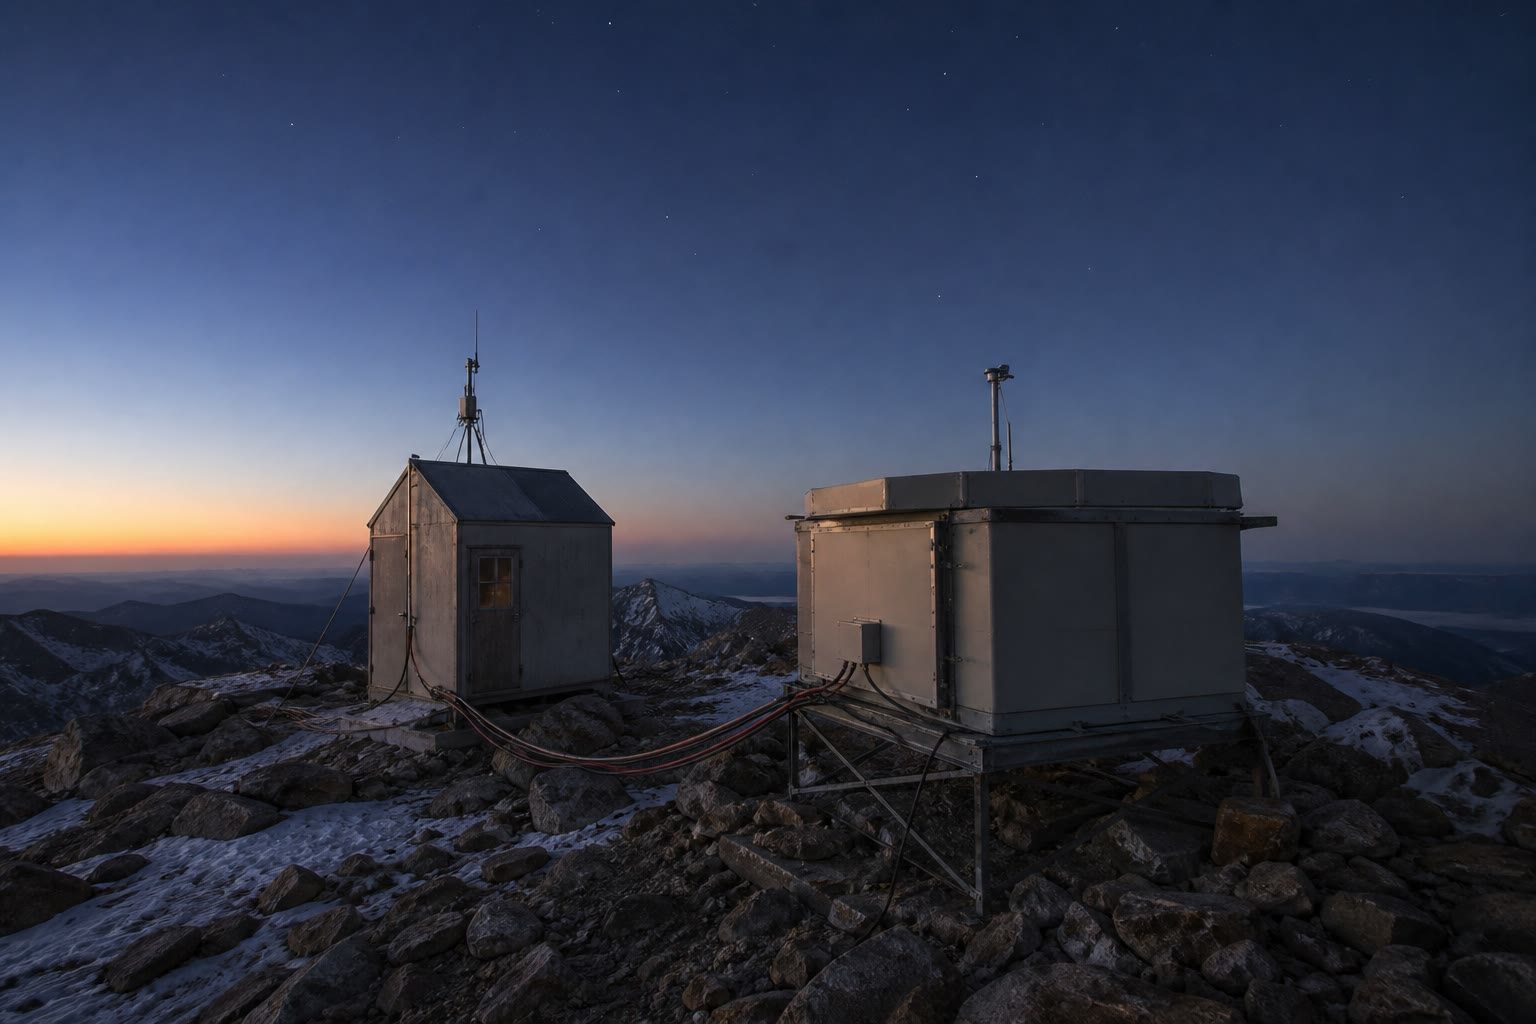
\includegraphics[width=0.58\linewidth]{images/book5/ai/b5-04-cosmic-ray-station.jpg}

{\small Een meetstation voor kosmische straling op hoogte. De muonen die het telt, tien kilometer hoger geboren, halen het alleen omdat bewegende klokken traag lopen --- \omterm{prop:b3:relativistic-kinematics:dilation}{tijdrek}, elke nacht op bergtoppen gemeten.}
\end{omfigure}

\section{Opgaven}

\begin{exercise}[$\star$]\label{exo:b3:relativistic-kinematics:1}
Bereken $\gamma$ voor $v/c = 0.1$, $0.5$, $0.9$, $0.99$ en $0.999$.
Bereken voor het ruimtestation ISS (\qty{7.7}{km/s}) de waarde van
$\gamma - 1$ met de benadering voor lage snelheden, en de tijd die de
bemanning per missie van zes maanden ``wint'' (of verliest?) ten opzichte
van een klok op de grond, zonder rekening te houden met zwaartekracht.
\end{exercise}

\begin{exercise}[$\star$]\label{exo:b3:relativistic-kinematics:2}
De lichtklok van de figuur: (a) schrijf de tik $\Delta\tau =
2d/c$ van de
klok in rust op ($d$ is de spiegelafstand); (b) leid met Pythagoras in het
stelsel waarin zij met $v$ beweegt $\Delta t =
\gamma\Delta\tau$ af; (c)
waarom eist het argument dat de dwarsafstand $d$ in beide stelsels
dezelfde is? (d) Geef het argument (twee identieke meetlatten die elkaar
passeren) waaruit volgt dat dwarslengten niet kunnen veranderen.
\end{exercise}

\begin{exercise}[$\star$]\label{exo:b3:relativistic-kinematics:3}
Een muon ontstaat op \qty{15}{km} hoogte met $v = 0.999c$. (a) Zijn
$\gamma$ en zijn gemiddelde levensduur in ons stelsel. (b) De gemiddelde
afstand die het aflegt. (c) De dikte van de atmosfeer in zijn stelsel.
(d) Welk deel van zulke muonen bereikt de grond, met en zonder
relativiteitstheorie (vervalwet $\eu^{-t/\tau}$, $\tau = \qty{2.2}{\micro s}$)?
\end{exercise}

\begin{exercise}[$\star$]\label{exo:b3:relativistic-kinematics:4}
Twee gebeurtenissen op de $x$-as: A in $(t = 0, x = 0)$, B in $(t =
\qty{2}{\micro s}, x = \qty{300}{m})$. (a) Bereken $\Delta s^2$:
tijdachtig of ruimteachtig? (b) Kan A de oorzaak van B zijn? (c) Bepaal de
snelheid van het stelsel waarin A en B op dezelfde plaats gebeuren, en de
\omterm{prop:b3:relativistic-kinematics:dilation}{eigentijd} ertussen in dat stelsel. (d) Dezelfde drie vragen voor B in
$(\qty{1}{\micro s}, \qty{600}{m})$ --- welk stelsel bestaat nu wel, en
welk niet?
\end{exercise}

\begin{exercise}[$\star\star$]\label{exo:b3:relativistic-kinematics:5}
GPS-satellieten draaien rond met $v = \qty{3.87}{km/s}$. (a) Bereken
$\gamma -
1$. (b) Hoeveel loopt een satellietklok per dag achter op een
klok op de grond, alleen door \omterm{prop:b3:relativistic-kinematics:dilation}{tijdrek}? (c) Plaatsbepaling werkt door
signalen met $c$ te timen: welke plaatsfout hoort bij één dag ongecorrigeerd
speciaal-relativistisch verloop? (d) De volledige correctie (met
zwaartekracht, in de geest van het slothoofdstuk behandeld) bedraagt
$+38\,\unit{\micro s}$ per dag, waarbij de zwaartekrachtsblauwverschuiving
het van de \omterm{prop:b3:relativistic-kinematics:dilation}{tijdrek} \emph{wint}: wat zegt het teken u over welk effect op
\qty{20200}{km} hoogte het grootst is?
\end{exercise}

\begin{exercise}[$\star\star$]\label{exo:b3:relativistic-kinematics:6}
(a) Een schip met $0.8c$ lanceert een sonde voorwaarts met $0.8c$ ten
opzichte van zichzelf: welke snelheid heeft de sonde voor ons? (b) Twee
schepen naderen elkaar, elk met $0.9c$ in ons stelsel: hun onderlinge
snelheid? (c) Toon uit de samenstellingswet aan dat uit $u' < c$ en $v < c$ volgt $u < c$ (ontbind de uitdrukking $c - u$). (d) Een laserpen die
over het gelaat van de maan strijkt kan een vlek schilderen die sneller
dan $c$ beweegt: waarom schendt dat geen enkele wet?
\end{exercise}

\begin{exercise}[$\star\star$]\label{exo:b3:relativistic-kinematics:7}
De natriumdubbellijn op \qty{589.0}{nm} komt van een ster aan op
\qty{575.0}{nm}. (a) Naderend of terugwijkend? Met welke snelheid? (b) Bij
welke snelheid zou zichtbaar licht (\qty{550}{nm}) naar het nabije
infrarood (\qty{1100}{nm}) verschuiven? (c) Toon voor $\beta \ll 1$ aan
dat $\Delta\lambda/\lambda \approx \beta$ en geef de vuistregel in km/s per
\unit{\angstrom} bij \qty{600}{nm}. (d) Een bron die op constante afstand
rondcirkelt vertoont een verschuiving zelfs zonder radiale beweging: welk
effect is dat, en van welke orde in $\beta$?
\end{exercise}

\begin{exercise}[$\star\star$]\label{exo:b3:relativistic-kinematics:8}
De polsstok en de schuur. Een polsstok van \qty{20}{m} wordt met $\gamma = 2$ naar een schuur van \qty{10}{m} met twee deuren gedragen. (a) De lengte
van de stok in het stelsel van de schuur: past hij? (b) In het stelsel van
de loper is de \emph{schuur} \qty{5}{m} lang: hoe kunnen beide gelijk
hebben? Benoem de twee gebeurtenissen (``voordeur sluit'', ``achterdeur
opent'') en vergelijk hun tijdsvolgorde in de twee stelsels. (c) Bereken de
tijd tussen deze gebeurtenissen in elk stelsel voor een sluiting die in de
schuur gelijktijdig is. (d) Geef de moraal in één zin (welke stilzwijgende
aanname maakte de ``paradox''?).
\end{exercise}

\begin{exercise}[$\star\star$]\label{exo:b3:relativistic-kinematics:9}
Een raket met \omterm{prop:b3:relativistic-kinematics:contraction}{eigenlengte} \qty{100}{m} passeert een ruimtestation met
$0.6c$. (a) Hoeveel tijd verstrijkt er op de klok van het station tussen
de passage van de neus en die van de staart? (b) Dezelfde vraag voor een
klok op de raket die het station (\omterm{prop:b3:relativistic-kinematics:contraction}{eigenlengte} \qty{300}{m}) voorbij ziet
gaan. (c) Het station schiet twee koppelklemmen gelijktijdig af (in zijn
stelsel), \qty{80}{m} uit elkaar: hoeveel tijd zit er voor de raket tussen
de twee schoten, en welke gaat het eerst af? (d) Ga na dat $\Delta s^2$
voor het paar klemgebeurtenissen in beide stelsels overeenkomt.
\end{exercise}

\begin{exercise}[$\star\star\star$]\label{exo:b3:relativistic-kinematics:10}
De tweeling, volledig. Stella vliegt met $0.8c$ naar een ster op
\qty{8}{ly} (in het aardstelsel) en keert met $0.8c$ terug; Terra blijft.
(a) Bereken de verstreken tijd van elk van beiden. (b) Hoe ver weg ligt de
ster in Stella's heenreisstelsel, en hoe lang duurt de heenreis voor haar?
(c) Wat berekent Stella vlak voor en vlak na het keerpunt voor ``de tijd
die het nu op aarde is'' (gebruik de term $vx/c^2$)? Toon aan dat haar
boekhouding bij de knik jaren verspringt --- en dat die sprong precies is
wat de totalen verzoent. (d) Leg uit waarom er vanuit Stella geen
symmetrisch argument te voeren is.
\end{exercise}

\begin{exercise}[$\star\star\star$]\label{exo:b3:relativistic-kinematics:11}
Lorentz eerlijk afgeleid. (a) Beredeneer uit de homogeniteit dat de
transformatie lineair moet zijn. (b) Leid, uitgaande van $x' = \gamma(x - vt)$ en, volgens het relativiteitsbeginsel, $x = \gamma(x' + vt')$, de
uitdrukking voor $t'$ in $t$ en $x$ af zonder licht te gebruiken. (c) Toon
aan dat de eis $x = ct \Rightarrow x' = ct'$ de $\gamma$ op de aangegeven
waarde vastlegt. (d) Waar precies gebruikte het argument elk postulaat?
\end{exercise}

\begin{exercise}[$\star\star\star$]\label{exo:b3:relativistic-kinematics:12}
Snelheidshoek. Definieer $\varphi$ door $\tanh\varphi = \beta$. (a) Toon
aan dat de \omterm{thm:b3:relativistic-kinematics:lorentz}{lorentztransformatie} luidt $ct' = ct\cosh\varphi - x\sinh\varphi$, $x' = x\cosh\varphi - ct\sinh\varphi$: een ``rotatie'' over
een imaginaire hoek, die $c^2t^2 - x^2$ behoudt zoals rotaties $x^2 + y^2$
behouden. (b) Toon aan dat het samenstellen van snelheden \emph{de
snelheidshoeken optelt}: $\varphi =
\varphi_1 + \varphi_2$, en vind de
samenstellingswet terug uit $\tanh(\varphi_1 + \varphi_2)$. (c) Een raket
versnelt met $g$ in haar eigen stelsel: bepaal, aannemend dat haar
snelheidshoek groeit als $\dd\varphi = g\,
\dd\tau/c$, de functie
$\beta(\tau)$ en hoeveel \omterm{prop:b3:relativistic-kinematics:dilation}{eigentijd} zij nodig heeft om $0.99c$ te halen.
(d) Waarom kan de snelheidshoek eeuwig groeien terwijl $\beta$ dat niet
kan?
\end{exercise}

\begin{omfigure}
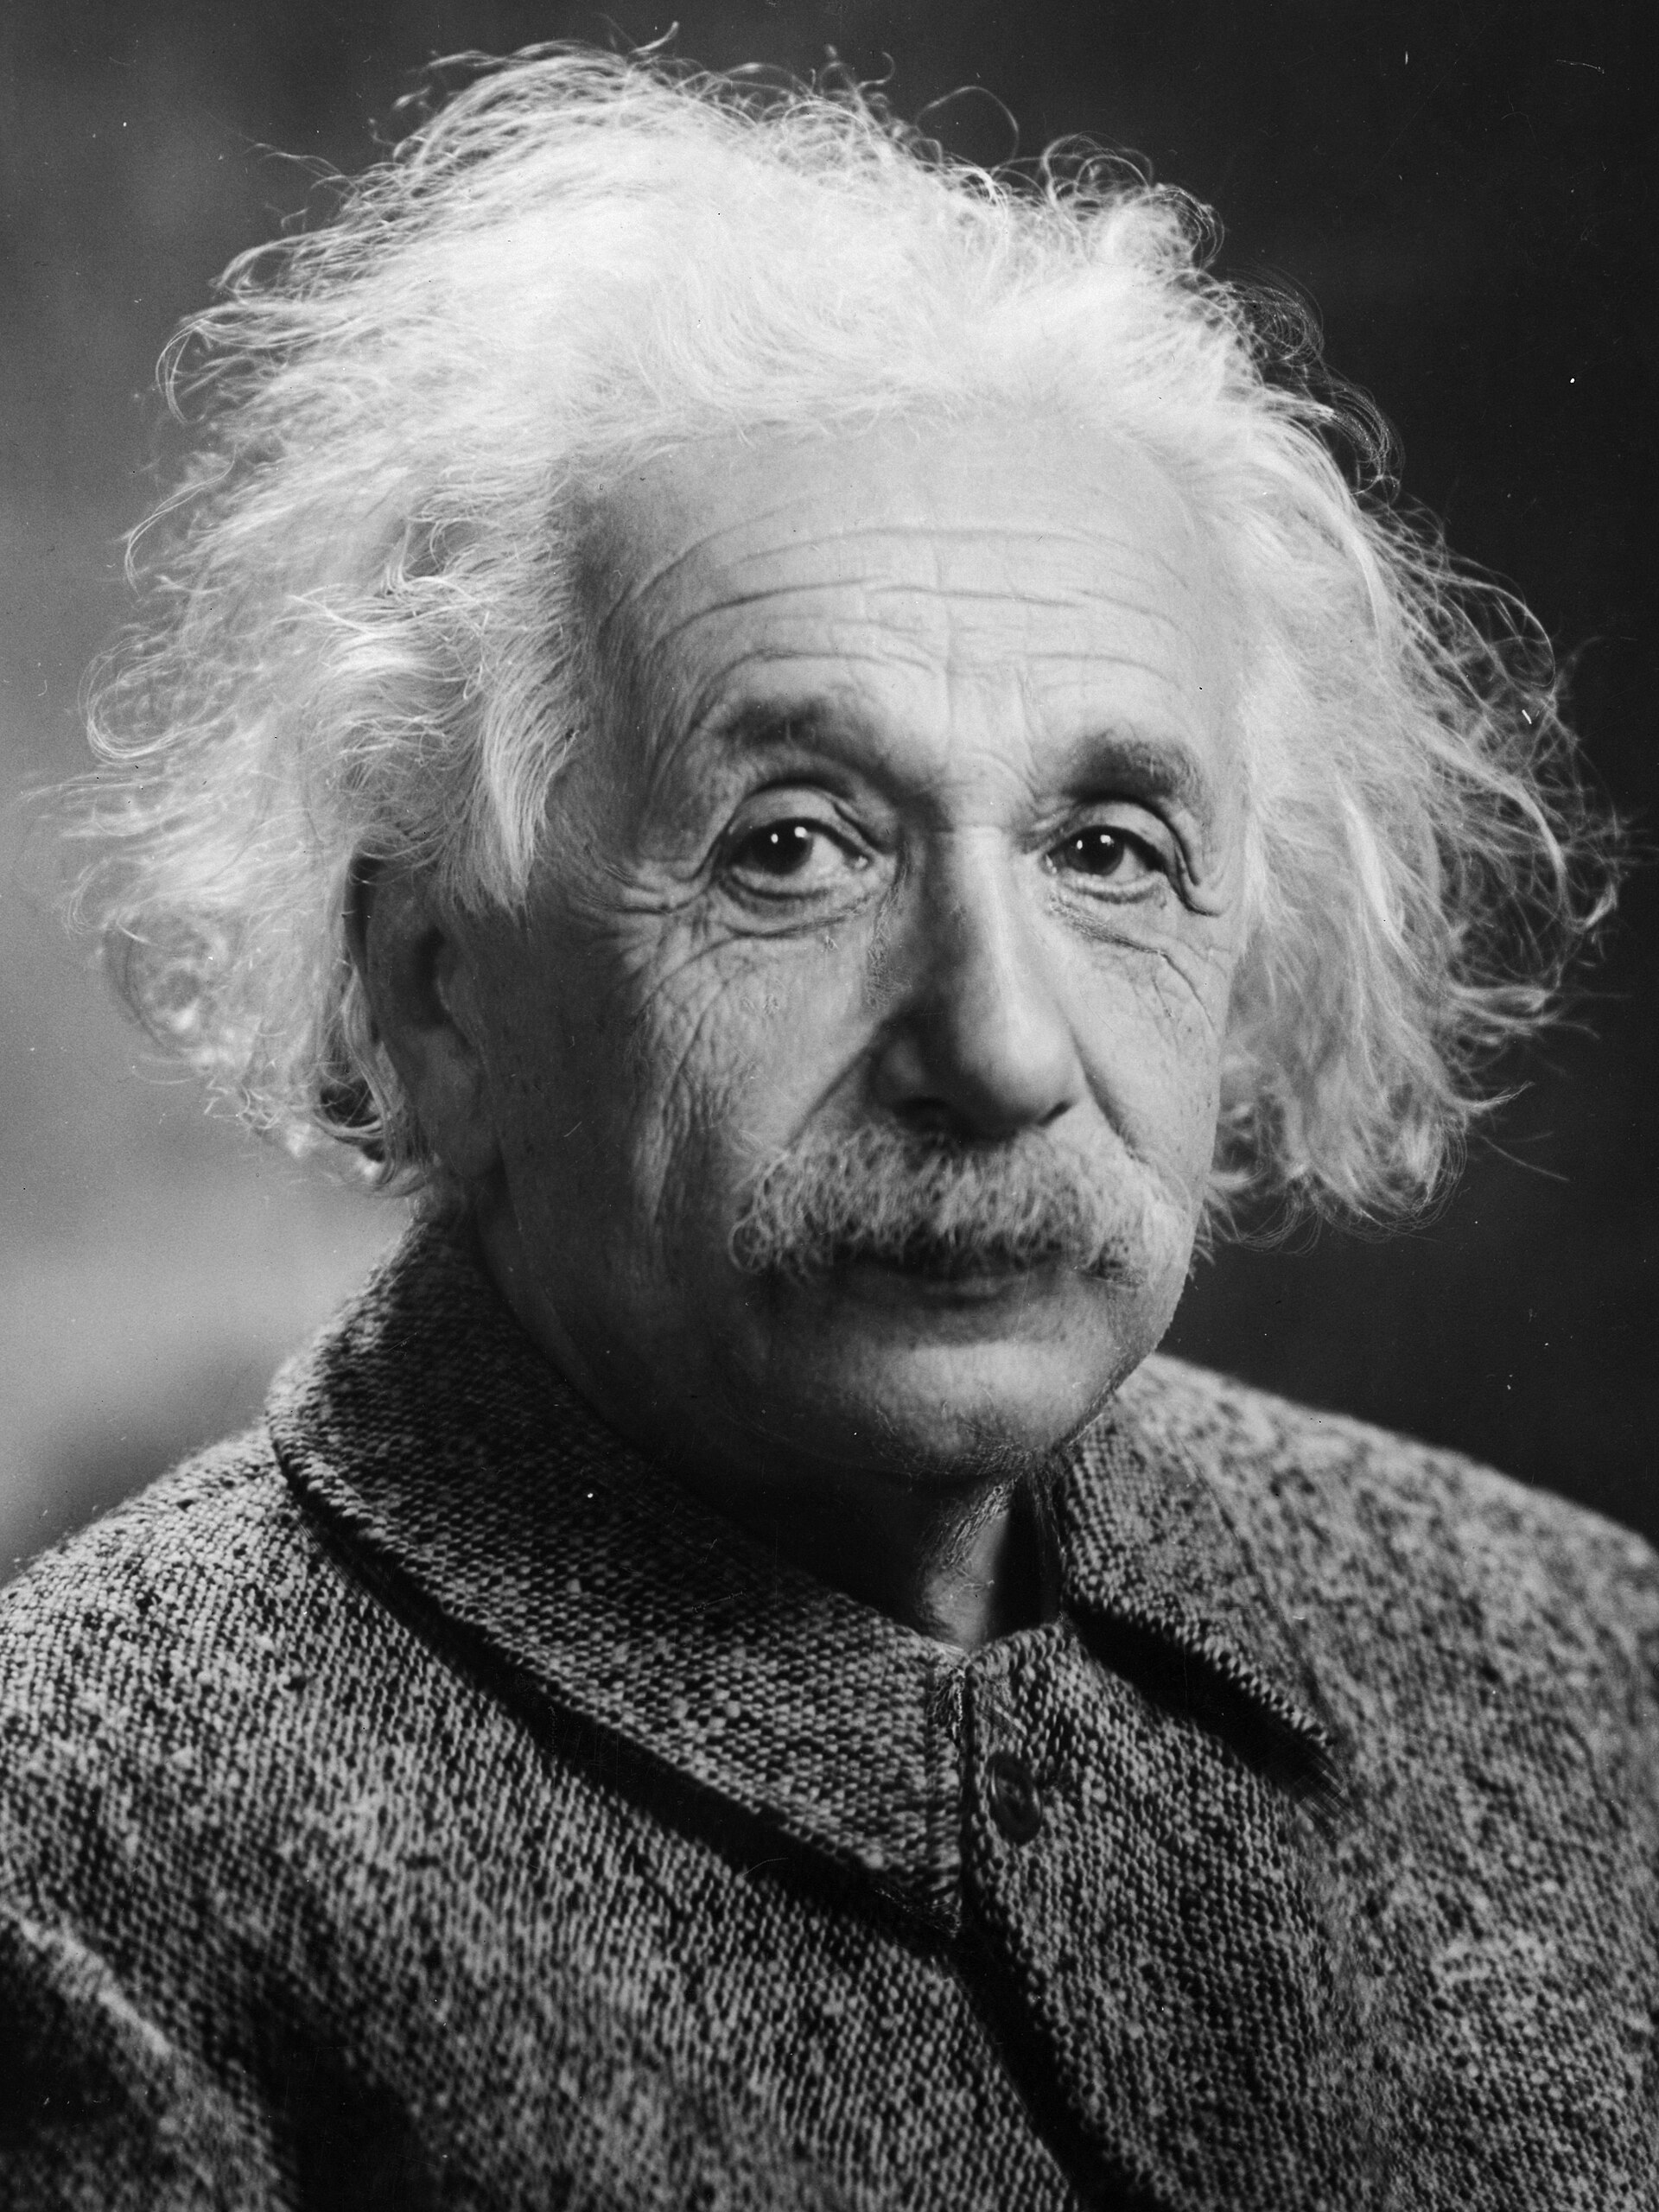
\includegraphics[width=0.34\linewidth]{images/book5/photo-einstein-1947.jpg}

{\small Albert Einstein (foto van Orren Jack Turner, 1947, publiek domein). Het relativiteitsartikel uit 1905 bouwde de kinematica opnieuw op uit twee postulaten --- dit hoofdstuk is, in wezen ongewijzigd, dat artikel met opgaven.}
\end{omfigure}

\section{Vraagstuk: Het experiment aan de hemel}

\begin{problem}[{Weekendvraagstuk --- muonen, bergklokken en het bewijs
dat de tijd rekt}]\label{pb:b3:relativistic-kinematics:1}
De zuiverste vroege toets van de \omterm{prop:b3:relativistic-kinematics:dilation}{tijdrek} gebruikte geen enkel
laboratoriumtoestel: de natuur levert relativistische klokken bij duizenden
en laat ze op elke berg regenen. Dit vraagstuk bouwt het experiment van
Frisch en Smith (1963) opnieuw op en brengt dezelfde natuurkunde dan omlaag
naar verkeersvliegtuigen en navigatiesatellieten. Gegevens: de gemiddelde
eigen levensduur van een muon is $\tau =
\qty{2.20}{\micro s}$; het verval
is exponentieel, waarbij een fractie $\eu^{-t/\tau}$ van de muonen een
\omterm{prop:b3:relativistic-kinematics:dilation}{eigentijd} $t$ overleeft; $c =
\qty{3.00e8}{m/s}$; Mount Washington:
hoogteverschil $h =
\qty{1907}{m}$ tussen de twee detectoren.

\medskip\noindent\textbf{Deel I --- Klokken die uit de hemel regenen.}
\begin{enumerate}
  \item Kosmische protonen treffen kernen hoog in de atmosfeer, en het
        puin vervalt op zo'n \qty{15}{km} hoogte tot muonen. Waarom is
        een populatie identieke onstabiele deeltjes een \emph{klok}?
  \item Bereken $c\tau$, het natuurlijke bereik van de gemiddelde
        levensduur van een muon.
  \item Welk deel van de muonen die op \qty{15}{km} ontstaan en met in
        wezen $c$ reizen zou zonder relativiteitstheorie de grond
        bereiken? (Geef de exponent; het getal zelf is absurd.)
  \item Detectoren op zeeniveau tellen muonen bij bosjes: formuleer de
        tegenspraak in één zin.
  \item De flux op zeeniveau bedraagt ongeveer één muon per vierkante
        centimeter per minuut: schat hoeveel muonen er elke seconde door
        uw uitgestrekte hand gaan, en door uw lichaam tussen twee
        hartslagen.
  \item Het experiment selecteerde muonen met snelheid $0.995c$: bereken
        hun $\gamma$.
  \item Frisch en Smith telden $563 \pm 10$ muonen per uur op de
        bergtop. Waarom meten op twee hoogten van dezelfde
        \emph{lawine} in plaats van op het ontstaansverhaal op
        \qty{15}{km} te vertrouwen?
\end{enumerate}

\medskip\noindent\textbf{Deel II --- De meting op de berg.}
\begin{enumerate}[resume]
  \item Hoe lang duurt de reis van \qty{1907}{m} met $0.995c$ in het
        stelsel van de berg?
  \item Welk deel overleeft die reis zonder \omterm{prop:b3:relativistic-kinematics:dilation}{tijdrek}, en hoeveel per uur
        zouden de onderste detector moeten bereiken?
  \item Hoeveel \emph{eigen} tijd verstrijkt er met \omterm{prop:b3:relativistic-kinematics:dilation}{tijdrek} voor het
        muon tijdens de reis?
  \item Voorspel met de relativiteitstheorie de overlevende fractie en
        het aantal per uur.
  \item De gemeten telling onderaan was $408 \pm 9$ per uur. Vergelijk
        beide voorspellingen met de meting en zeg welke theorie haar
        ontmoeting met de berg overleeft.
  \item Haal uit de gemeten verhouding $408/563$ de
        \emph{experimentele} rekfactor en vergelijk hem met $\gamma = 10$. (De muonen worden in de gesteenteachtige afscherming iets
        afgeremd, zodat de effectieve $\gamma$ iets onder de waarde op
        de bergtop ligt --- Frisch en Smith vonden $8.8 \pm
        0.8$.)
\end{enumerate}

\medskip\noindent\textbf{Deel III --- Het verhaal van het muon zelf.}
\begin{enumerate}[resume]
  \item Hoe hoog is Mount Washington in het stelsel van het muon?
  \item Hoe lang doet de berg erover om voorbij te stromen, en welk deel
        van de muonen vervalt in die tijd? Ga na dat dit klopt met de
        voorspelling van deel II.
  \item De twee stelsels zijn het oneens over wat er rekte (onze tijd?\
        zijn berg?) en toch eens over de telling: van welke soort is de
        telling als grootheid, en waarom moeten alle stelsels het erover
        eens zijn?
  \item Bereken het interval $\Delta s^2$ tussen het ontstaan bovenaan
        en de aankomst onderaan in het stelsel van de berg, en ga na dat
        $\Delta s/c$ gelijk is aan de \omterm{prop:b3:relativistic-kinematics:dilation}{eigentijd} van het muon uit deel
        II.
  \item Een scepticus werpt tegen: ``misschien verandert de hoogte de
        vervalsnelheid, en niet de snelheid.'' Welke controle levert de
        gemeten afhankelijkheid van $\gamma$ (tragere muonen rekken
        minder)?
  \item Moderne opslagringen houden muonen bij $\gamma = 29.3$ vast en
        meten levensduren tot op $\num{e-3}$: wat vinden zij, en wat
        voegt een cirkelbaan aan de toets toe (welk lid van de tweeling
        is het muon)?
\end{enumerate}

\medskip\noindent\textbf{Deel IV --- Terug op aarde: vliegtuigen en
satellieten.}
\begin{enumerate}[resume]
  \item Een verkeersvliegtuig kruist met \qty{250}{m/s} op een vlucht van
        \qty{40}{h} rond de wereld. Bereken met $\gamma - 1 \approx v^2/2c^2$ de speciaal-relativistische achterstand van zijn klok,
        in nanoseconden.
  \item Cesiumklokken zien nanoseconden moeiteloos; de vluchten van 1971
        bevestigden de voorspelling (zodra de tegengestelde duw van de
        zwaartekracht, groter op hoogte, was meegenomen). Waarom moeten
        de twee effecten worden gescheiden door \emph{zowel} oostwaarts als
        westwaarts te vliegen?
  \item Welke speciaal-relativistische achterstand bouwt een
        GPS-satelliet ($v = \qty{3.87}{km/s}$) per dag op, in
        microseconden?
  \item Hoeveel kilometer afstandsfout zou \emph{één week} van dat
        verloop alleen ongecorrigeerd opleveren?
  \item De volledige GPS-correctie, $+38\,\unit{\micro s}$ per dag met
        zwaartekracht meegerekend, wordt vóór de lancering in de
        satellietklokken ingebouwd: wat zou een navigator binnen enkele
        uren merken als dat niet gebeurde?
  \item Vat het genoemde resultaat samen: een berg, twee tellers en
        klokken van $2.2\,\unit{\micro s}$ maten in 1963 de \omterm{prop:b3:relativistic-kinematics:dilation}{tijdrek} bij
        $\gamma \approx 9$ tot op $10\%$ --- en voor dezelfde natuurkunde
        wordt elke seconde gecorrigeerd, in elke telefoon die weet waar
        zij is.
\end{enumerate}
\end{problem}
